\documentclass[conference]{IEEEtran}
\IEEEoverridecommandlockouts
% The preceding line is only needed to identify funding in the first footnote. If that is unneeded, please comment it out.
\usepackage{cite}
\usepackage{amsmath,amssymb,amsfonts}
\usepackage{algorithmic}
\usepackage{graphicx}
\usepackage{textcomp}
\usepackage{xcolor}
\def\BibTeX{{\rm B\kern-.05em{\sc i\kern-.025em b}\kern-.08em
    T\kern-.1667em\lower.7ex\hbox{E}\kern-.125emX}}
\begin{document}

\title{Identification of Digits from Sign Language Images}

\author{\IEEEauthorblockN{José Santos, 98279}
\IEEEauthorblockA{\textit{DETI} \\
\textit{Universidade de Aveiro}}
\and
\IEEEauthorblockN{Henrique Sousa, 98324}
\IEEEauthorblockA{\textit{DETI} \\
\textit{Universidade de Aveiro}}
}

\maketitle

\begin{abstract}
    The purpose of this work is to implement and
    compare machine learning models capable of identifying digits from sign language images.
    In this paper, we tried to obtain a good result with the models using
    a dataset provided by Kaggle. Some changes are discussed,
    based on the work of others that positively affected our
    work.
\end{abstract}

\begin{IEEEkeywords}
Sign language recognition, Digit recognition, Machine learning
\end{IEEEkeywords}

\section{Introduction}
In recent years, there has been growing interest in using machine learning to develop computer vision systems capable of recognizing sign language gestures. Such systems could be used to improve communication between hearing and non-hearing individuals, as well as to facilitate the development of new technologies for the deaf and hard-of-hearing community.

In this paper, we present a novel approach to digit recognition from sign language images using machine learning. We explore several different models, including neural networks, support vector machines, and decision trees, and compare their performance on a dataset of sign language images. We also investigate the impact of some preprocessing techniques.

\section{State of the art}
Over the past few years, there have been several studies and projects focused on recognition from sign language images using machine learning techniques. Many of these approaches have utilized deep learning methods such as convolutional neural networks (CNNs), which have been shown to be effective in image recognition tasks.

\textcolor{red}{TODO: Add some references to the state of the art}
\section{Dataset Analysis}
For the development of this work, we used a dataset provided by Kaggle that contains 2062 images of sign language digits. The dataset is well balanced, with a minimum of 204 examples for a label and a maximum of 208, ensuring that every label has a similar number of examples (Figure \ref{fig:dataset-balanced}). The dataset includes data for the digits 0 to 9, resulting in 10 labels in total as we can see on the figure \ref{fig:dataset-examples}. 

\begin{figure}[h]
    \centering
    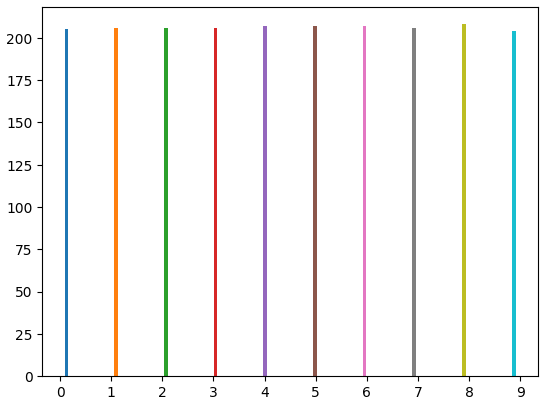
\includegraphics[width=0.4\textwidth]{assets/dataset-labels.png}
    \caption{Dataset balanced distribution}
    \label{fig:dataset-balanced}
\end{figure}


\begin{figure}[h]
    \centering
    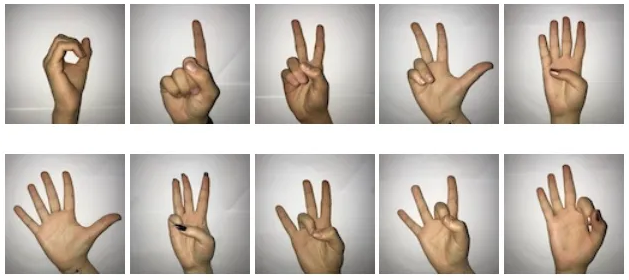
\includegraphics[width=0.4\textwidth]{assets/sign-language-digits.png}
    \caption{Dataset label examples}
    \label{fig:dataset-examples}
\end{figure}

The images are provided in a \textit{.npy} format, but we found it easier to work with the raw images to manipulate them and apply preprocessing techniques to improve the model's performance. The dataset's size and balanced distribution make it an ideal choice for training and evaluating machine learning models for digit recognition from sign language images.

\section{Dataset Preprocessing}

\subsection{Image Augmentation}
The first thing we did to the images was to augment them in order to create more data for training. 
We used the \textit{imgaug.augmenters} to perform the augmentation. 
The following changes were made to the images:
\begin{itemize}
    \item \textit{\textbf{Rotate}} - Rotate the image by a random angle between -20 and 20 degrees.
    \item \textit{\textbf{Gaussian noise}} - Add gaussian noise with standard deviation of 0 to 0.05*255
    \item \textit{\textbf{Gamma contrast}} - Change the contrast of the image by a random factor between 0.5 and 1.5.
\end{itemize}
For every image in the dataset, we created 5 new images with the above changes. Due to the small size of the dataset, we decided to perform the augmentation offline, before splitting the dataset into training and test data.

\subsection{Image Preprocessing}
We also resized the images to 50x50 pixels (down from the original size of 64x64), as we found that this size was sufficient for the models to achieve good results. Then, we converted the images to grayscale and flattened them, as we found that this improved the performance of the models.

Finally, we split the dataset into training and test data. We used a 80/20 split, with 80\% of the data being used for training and 20\% for testing.
Resulting in 9897 total images for the training data and 2475 for the test data.
\section{Models}

\section{Conclusion}

\section{References}

\begin{thebibliography}{00}
    \bibitem{b1} Akanksha Telagamsetty, Sign Language Digits Classification https://medium.com/analytics-vidhya/sign-language-classification-64fe8ad0fc2c
\end{thebibliography}

\end{document}
